\let\negmedspace\undefined
\let\negthickspace\undefined
\documentclass[journal,12pt,onecolumn]{IEEEtran}
\usepackage{cite}
\usepackage{amsmath,amssymb,amsfonts,amsthm}
\usepackage{algorithmic}
\usepackage{graphicx}
\graphicspath{{./figs/}}
\usepackage{textcomp}
\usepackage{xcolor}
\usepackage{txfonts}
\usepackage{listings}
\usepackage{enumitem}
\usepackage{mathtools}
\usepackage{gensymb}
\usepackage{comment}
\usepackage{caption}
\usepackage[breaklinks=true]{hyperref}
\usepackage{tkz-euclide} 
\usepackage{listings}
\usepackage{gvv}                                        
%\def\inputGnumericTable{}                                 
\usepackage[latin1]{inputenc}     
\usepackage{xparse}
\usepackage{color}                                            
\usepackage{array}
\usepackage{longtable}                                       
\usepackage{calc}                                             
\usepackage{multirow}
\usepackage{multicol}
\usepackage{hhline}                                           
\usepackage{ifthen}                                           
\usepackage{lscape}
\usepackage{tabularx}
\usepackage{array}
\usepackage{float}
\newtheorem{theorem}{Theorem}[section]
\newtheorem{problem}{Problem}
\newtheorem{proposition}{Proposition}[section]
\newtheorem{lemma}{Lemma}[section]
\newtheorem{corollary}[theorem]{Corollary}
\newtheorem{example}{Example}[section]
\newtheorem{definition}[problem]{Definition}
\newcommand{\BEQA}{\begin{eqnarray}}
\newcommand{\EEQA}{\end{eqnarray}}
\newcommand{\define}{\stackrel{\triangle}{=}}
\theoremstyle{remark}
\newtheorem{rem}{Remark}

\begin{document}

\title{2.5.19}
\author{ee25btech11056 - Suraj.N}
\maketitle
\renewcommand{\thefigure}{\theenumi}
\renewcommand{\thetable}{\theenumi}

\textbf{Question} : Find the value of $p$ for which the lines $\dfrac{1-x}{3}=\dfrac{2y-14}{2p}=\dfrac{z-3}{2}$ and $\dfrac{1-x}{3p}=\dfrac{y-5}{1}=\dfrac{6-z}{5}$ are perpendicular.

\textbf{Solution:}

\begin{table}[h!]
  \centering
  

  \caption*{Table : Lines}
  \label{2.5.19}
\end{table}


These lines can also be written in the vector form $\vec{x}=\vec{h}+k\vec{m}$ .

\begin{align*}
  \text{Line A: }\;\; \vec{x}=\myvec{1\\7\\3}+k_1\myvec{-3\\p\\2} \\
  \text{Line B: }\;\; \vec{x}=\myvec{1\\5\\6}+k_2\myvec{-3p\\1\\-5}
\end{align*}

Hence, the direction vectors are
\begin{align*}
  \vec{m_1}=\myvec{-3\\ p\\ 2}, \qquad
  \vec{m_2}=\myvec{-3p\\ 1\\ -5}.
\end{align*}

For the lines to be perpendicular, we require $\vec{m_1^\top} \vec{m_2}=0$.

\begin{align*}
  \vec{m_1^\top} \vec{m_2}
&= \myvec{-3 & p & 2}\myvec{-3p\\ 1\\ -5} \\
&= (-3)(-3p) + p(1) + 2(-5) \\
&= 9p + p - 10 \\
&= 10p - 10.
\end{align*}

Thus,
\begin{align*}
10p - 10 = 0 \;\Rightarrow\; p=1.
\end{align*}

\textbf{Final answer:} $p=1$.

\pagebreak

\begin{figure}[h!]
  \centering
  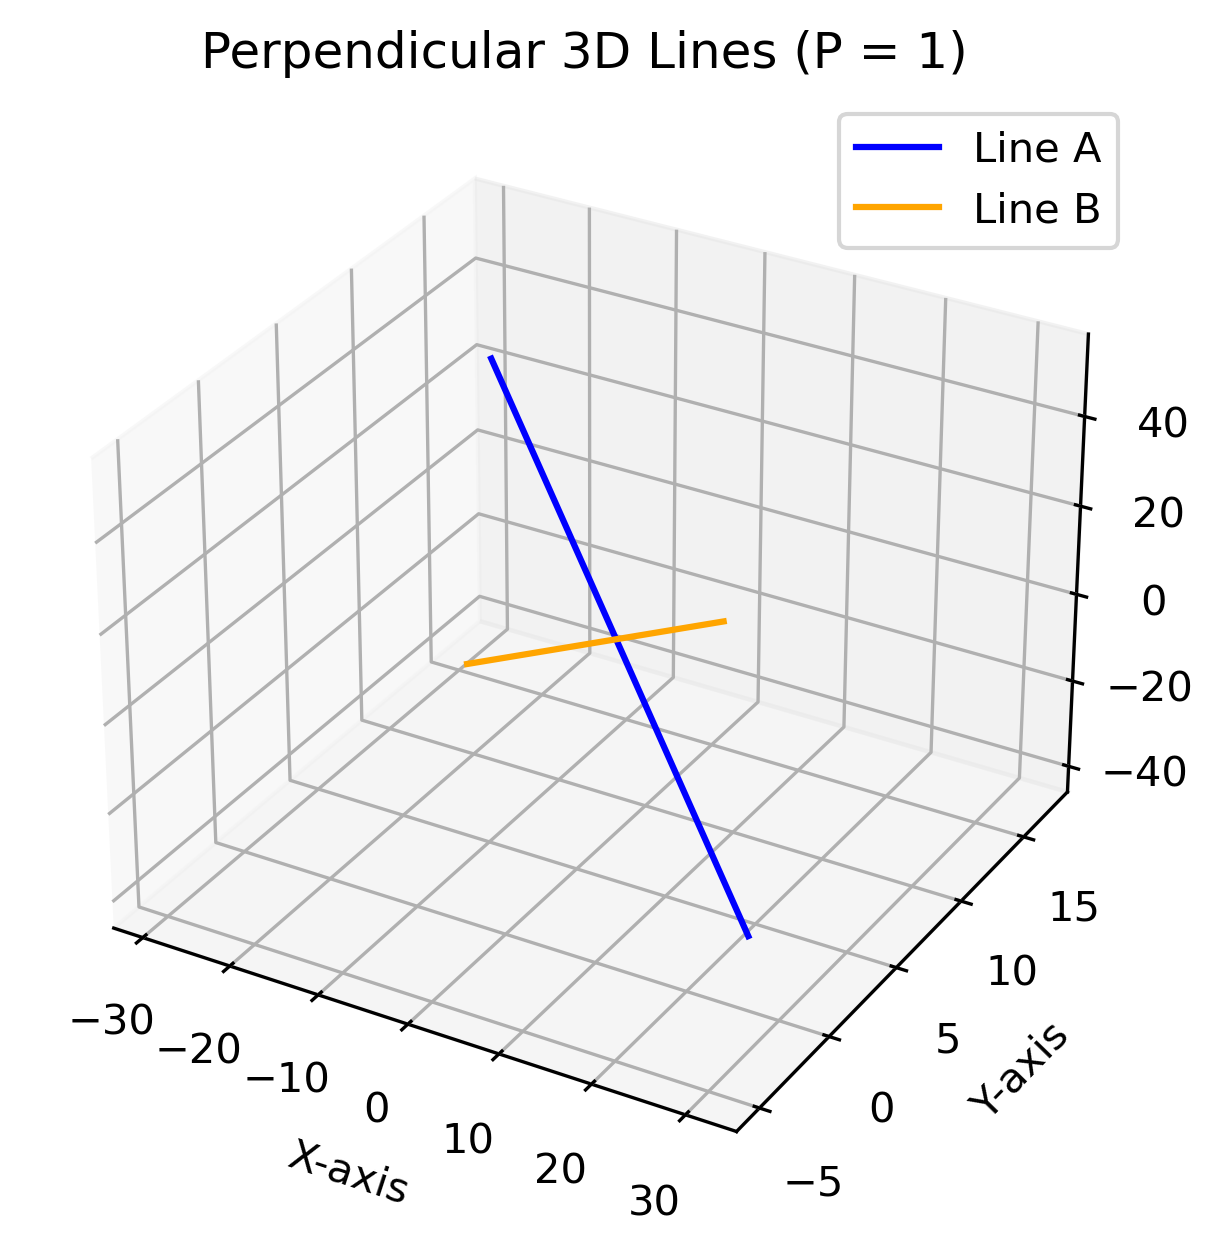
\includegraphics[width=0.9\columnwidth]{figs/perpendicular_lines.png} 
   \caption*{Fig : Lines A and B}
  \label{Fig1}
\end{figure}


\end{document}
